\lhead{\emph{Active Magnetic Field Compensation Prototype}}
\chapter{Active Magnetic Field Compensation Prototype}\label{ch:amcP}
% \printinunitsof{pt}\prntlen{\textwidth}

In Chapter~\ref{ch:magnetics}, the requirements of the magnetic field for nEDM experiment have been discussed. It also includes the active magnetic compensation to stabilize the external magnetic field. This thesis is based on the development of Active Compensation system for the TUCAN nEDM experiment. For that purpose a prototype has been built and tested at University of Winnipeg. This chapter describes the different components needed to make the prototype successfully running. It starts with giving an overall overview of the prototype and then move into describing every components in details. Finally, the chapter ends with giving an idea about the surrounding field fluctuations around the prototype experimental setup. In Chapter~\ref{ch:operation}, we then move into discussing the feedback algorithm needed to make the prototype working as active compensation.

The first section in this chapter gives an overview of the prototype which is presented next.


% The chapter describes the Active Magnetic Field Compensation (AMC) prototype that has been built at the University of Winnipeg. All the apparatus that made the AMC prototype will be discussed in detail.

\section{Overview of AMC Prototype}\label{sec:amcp_overview}
This Section gives an overview of the AMC prototype that has been built at the University of Winnipeg in the development process of implementing the original one at TUCAN nEDM experiment.

The magnetic background fluctuation has been found to be $\sim$ 100 nT (see section \ref{sec:field}) over a full day. The prototype has been designed to compensate that by introducing six current carrying closed loop coils on six faces of a cube surrounding the outermost mu-metal shield of a four layer cylindrical passive shielding enclosing the imaginary experimental area. To see how well the prototype response for a constant perturbation, an electro-magnet coil has also been used. The properties of mu-metal shields have been discussed more in Section~\ref{sec:shield} and the coil cube in Section~\ref{sec:cube}. The full prototype with different apparatus has shown in terms of schematic diagram in Fig.~\ref{fig:active}\textcolor{blue}{(a)} and also a glimpse of the actual experiment was shown in Fig.~\ref{fig:active}\textcolor{blue}{(b)}.

There are four 3-axis fluxgate sensors placed at different positions within the compensation coils to measure field for compensation and one 3-axis fluxgate sensor placed at the center of the origin of the prototype for quantification of the prototype. A breakout box was built to separate each of $x$, $y$ and $z$ axis in respective direction and provide power. More about the fluxgate sensors have been discussed in Section~\ref{sec:sensor}.

\doublefig{Images/exp3}{width =\textwidth,height =8cm}{Schematic diagram \label{fig:exp}}{Images/exp_photo}{width = \textwidth,height =8cm}{Photograph\label{fig:exp_photo}}{{Active Magnetic Field Compensation (AMC) Prototype at University of Winnipeg. The schematic diagram with different apparatus is shown in (a) and the actual experiment photograph is shown in (b). Surrounding the outermost mu-metal passive shielding layer, there are six coils on six faces. There is another elctro-magnet coil working as perturbation coil. The magnetic environment is sensed by the 3-axis fluxgates placed in different positions on the surface of the coils where $x$, $y$ and $z$ axis have been separated by a breakout box. A fourth order low pass Butterworh filter has been built  to get rid of high frequency noise. For signals transferring to and from computer, analog to digital converter (ADC) and digital to analog converter (DAC) of LabJack T7 Pro have been used. Six current sinks circuits generate the required currents that are sent to the six coils. } \label{fig:active}}{Active Magnetic Field Compensation (AMC) Prototype at University of Winnipeg}


\FloatBarrier
\clearpage
The fluxgates suffer from environmental noise in terms of 60 Hz electrical noise due to grid line transmitted from power station and others. Therefore, a $\mathrm{4^{th}}$ order low pass Butterworth filter with corner frequency at 10 Hz has been built to try to reduce the noise. The filter details are in Section~\ref{sec:filter}. After filtering, the signals are transmitted to the computer via analog to digital converter (ADC) of LabJack T7 Pro where required currents are calculated via proportional integral (PI)for control algorithm. The information for required currents are sent from computer to 6 voltage controlled current source circuits termed as current sinks. Finally, the current generated by the current sinks are sent to the six compensation coils for reducing the drift in the fluxgate signals.  via digital to analog converter (DAC).

% \fig{Images/exp2}{width = 0.8\textwidth}{Schematic diagram of prototype active compensation system at University of Winnipeg.\label{fig: active}}
The above discussion  has given an idea about the different apparatus that made the prototype. Next each of them will be discussed in details starting with  the mu-metal passive shields.

\section{Mu-Metal Shields}\label{sec:shield}
Generally, the passive magnetic shielding as explained in Section \ref{sec:passive} is composed of a thin multi-layer shields with materials having high magnetic permeability such as mu-metal. The outer layers are usually cylindrical \cite{mu_cyl_1,mu_cyl_2} but they can also take the same forms as the magnetic shielded room (msr)~\cite{mu_msr_1,mu_msr_2}. The inner layer is designed based on the coil to achieve required homogeneity \cite{mu_inner_1,mu_inner_2}. 

\fig{Images/passive}{width = \textwidth}{Prototype passive shielding at University of Winnipeg. Inner cylinder is shown in (a), (b) shows 4 mu-metal cylindrical shields of passive shielding by OPERA simulation software and (c) shows photograph of 3 layers of prototype passive shielding. The outer layer is not shown in (c).\label{fig: passive}}{Prototype passive shielding at University of Winnipeg}


However, in the prototype, there are four layers of cylindrical shields enclosing the imaginary experimental area with end-caps on them. The prototype passive shielding at University of Winnipeg is shown in Fig.~\ref{fig: passive}. The inner cylinder with end caps is shown in Fig.~\ref{fig: passive}\textcolor{blue}{(a)}. All the 4 layers are shown in Fig.~\ref{fig: passive}\textcolor{blue}{(b)} by OPERA simulation software and the software itself has been explained in detail in Section~\ref{fig:opera_setup}. A photograph of 3 layers excluding the outermost layer of prototype passive shielding is shown in Fig.~\ref{fig: passive}\textcolor{blue}{(c)}. Amumetal (Magnifer 7904) of thickness 0.0625 inch has been used for the layers,  which is an 80\% Nickel-Iron alloy and was fabricated and annealed by Amuneal Manufacturing Corp \cite{mu-metal}.  There are two end-caps in each cylinder with a 7.5 cm diameter in the central hole. And to minimize the leakage of the external fields into the progressively shielded inner volumes, a stove-pipe of length 5.5 cm is placed on each hole. One of the stove-pipe of the inner cylinder is seen in Fig.~\ref{fig: passive}\textcolor{blue}{(a)}. The radius and length of the four layers including the stove pipes are shown in Table \ref{table:mu-metal}. The center of the enclosed area is the center of the origin of the prototype. A combined DC shielding factor of the order of $\mathrm{10^6}$ is expected. A discussion about another prototype of similar design but smaller in size can be found in Ref. \cite{baby_shield}.

\begin{table} [!htb]
    \centering
    \begin{tabular} { |c|c|c|c|c|c|} 
        \hline
        Parameters & Innermost Layer & $\mathrm{2^{nd}}$ Layer & $\mathrm{3^{rd}}$ Layer & Outermost Layer & Stove Pipe\\
        \hline\hline
        Radius (cm) & 18.5 & 23.5 & 30 & 38 & 3.7 \\ 
        \hline
        Length (cm) & 37 & 55 & 71 & 90 & 5.5 \\ 
         \hline
    \end{tabular}
    % \vspace{4mm}
    \caption[Dimensions of prototype passive shielding layers]{Dimensions of prototype passive shielding layers including stove pipes radius and length.}\label{table:mu-metal}
\end{table}

\FloatBarrier
The above discussion gives an idea about the dimensions and properties of the prototype passive shielding at the University of Winnipeg. Next the coil cube will be discussed in details.

\section{Coil Cube}\label{sec:cube}
As discussed in Section ~\ref{sec:amcp_overview}, the prototype has been designed to compensate $\sim 100$ nT (see section \ref{sec:field}) magnetic background fluctuations over a full day by introducing six current carrying closed loop coils on six faces of a cube surrounding the outermost mu-metal shield. The coils are termed as $C_x^\pm$, $C_y^\pm$ and $C_z^\pm$ respectively and known as compensation coils as they are responsible for compensating the magnetic fluctuations. The opposite face coils are separated by 1.15 m taking relatively similar shape as  Helmholtz coils. In addition to those, there is also a perturbation electro-magnet coil namely $P_z^+$. The coil configuration is shown in Fig.\ref{fig: coil}. The numbers 1-8 indicating the postions of the fluxgate sensors which will be discussed in the next section.

\fig{Images/coil}{width = \textwidth}{Schematic diagram indicating the coil   configuration and the position of the fluxgate sensors.\label{fig: coil}}{Schematic diagram indicating the coil configuration and the position of the fluxgate sensors.}


\FloatBarrier
The compensation coils have been chosen to be single turn to have small resistance ($\sim$ 0.15 $\Omega$) and small inductive reactance that oppose the reduction of the current flow in them. The have the dimensions of 1.15 m$\times$1.15 m. The perturbation electro-magnet coil has also the same dimension as the compensation coils but it has 77 no. of turns. The perturbation coil was typically placed in the same face as $C_z^+$ and separated from it by 1.06 m. The coils properties are shown by Table \ref{table:coil}. 

\begin{table} [!htb]
    \centering
    \begin{tabular} { |c|c|c| } 
        \hline
        Parameters & \makecell{Compensation Coils \\ ($C_x^\pm$, $C_y^\pm$ and $C_z^\pm$)} & \makecell{Perturbation Coil \\ ($P_z^+$)} \\
        \hline\hline
        Dimension (m$\times$m) & 1.15$\times$1.15 & 1.15$\times$1.15\\ 
        \hline
        No. of Turns & 1 & 77\\ 
        \hline
        Resistance ($\Omega$) & 0.15 & 11.55\\ 
        \hline
        Inductance (mH) & 0.32 & 24.62\\
        % \hline
        % Current ($A$) & 0 & 1\\
         \hline
    \end{tabular}
    % \vspace{4mm}
    \caption{Coils dimension and properties.}\label{table:coil}
\end{table}

\FloatBarrier
The above discussion gives an idea about the coil configuration, dimensions and properties. Next, the apparatus used to measure magnetic field will be discussed.


\section{Fluxgate Sensors}\label{sec:sensor}

A fluxgate sensor is a piece of magnetic material, within a sensing winding used for measuring the magnitude and direction of DC or low-frequency ac magnetic fields. The magnetometer$'$s sensitivity direction is the axis of the sensing winding. The magnetic material is periodically saturated by a source of excitation power. It is the transition of this material into magnetic saturation that creates the measurement signal.

For the prototype, we have used four 3-axis fluxgate sensors (2 Bartington Mag-03 and 2 Bartington Mag690) placed at different positions within the compensation coils to measure field for compensation. Beside those, one 3-axis fluxgate sensor (Bartington Mag690) has been placed at the center of the origin of the prototype for quantification of the prototype. The numbering 1-8 in Fig.~\ref{fig: coil} indicate the positions of the possible placements of the fluxgates from where the magnetic fields have been measured. Note that, we have also tried more positions other than that are shown on that figure which will be discussed in Chapter~\ref{ch:quantification}.  The measured data from the fluxgate sensors are transferred to the computer via anlog to digital converter (ADC) of LabJack T7 Pro which will be discussed in the next section. But before coming to the ADC, the 3-axis of the fluxgates have to be separated and for that purpose we have build  2 breakout boxes. Each of the breakout boxes can separate four 3-axis fluxgate sensors that means each can provide the data for 3$\times$4=12 sensors. The the 3-axis directions of the fluxgate sensors are shown in Fig.~\ref{fig: coil} by the label X, Y and Z which represent the $x$, $y$ and $z$ axis of a fluxgate.  The properties of the fluxgate sensors that we have used for the prototype are shown in Table~\ref{tablE:sensor} and collected from the Bartington's (manufacturer) website~\cite{flux}. 

\begin{table} [!htb]
    \centering
    \begin{tabular} { |c|c|c|c|c|c|} 
        \hline
        Parameters & Mag-03 & Mag690 \\
        \hline\hline
        Measure Range ($\mu$T) & $\pm$70 & $\pm$100 \\ 
        \hline
        \makecell{Noise Level \\($\mathrm{pT_{rms}\;/\sqrt{Hz}}$ at 1 Hz)} & $<$6 & 10$-<$20 \\ 
        \hline
        Bandwidth (kHz) & 3 & 1 \\ 
        \hline

    \end{tabular}
    % \vspace{4mm}
    \caption{Properties of the fluxgate sensors used for the prototype.}\label{tablE:sensor}
\end{table}

\FloatBarrier
According to the manufacturer (Bartington), the typical noise levels are from $\mathrm{10}$ to $\mathrm{<20\;pT_{rms}\;/\sqrt{Hz}}$ and $\mathrm{<6 \; pT_{rms} \;/\sqrt{Hz}}$ at $\mathrm{1}$ Hz for Mag690 and Mag-03 respectively. The noise levels of the fluxgates had been tested  and were found to match the manufacturer standard. For that, data was taken by placing Mag690 and Mag03 fluxgates inside the shield at different times. Then the data was processed in Mathematica \cite{Mathematica} to estimate the power spectral density using Discrete Fourier Transform (DFT) \cite{dft}. The Fig.~\ref{fig:noise} shows that the noise level is $\sim$ $\mathrm{16\;pT_{rms}\;/\sqrt{Hz}}$ at $\mathrm{1}$ Hz for Mag690. It confirms that ADC doesn't present noise beyond fundamental noise of fluxgate.

\fig{Images/noise}{width =  \textwidth}{Average Spectral Density for Mag690. \label{fig:noise}}{Average Spectral Density for Mag690.}


The above discussion gives an idea about the definition of the fluxgate sensor and the properties of the fluxgate sensors that we hav used. Next in the list according to Fig.~\ref{fig:active}\textcolor{blue}{(a)}, we should discuss the filter. But the necessity of the filter came later and so the data acquisition process will be discussed  where the analog to digital converter (ADC) and digital to analog converter (DAC) are the main components.


\section{Data Acquisition (DAQ) Module}\label{sec:DAQ}

The signals that we get from the fluxgates are all analog which we have to sent to the computer to process the signals by PI control algorithm. But the computer doesn$'$t understand analog signal rather it works on digital signal. So, we need a converter that will transform our analog signal to the digital one. Again, the siganls that are processed by PI control algorithm in computer must send to the coils. So, we also need a converter that will transform the digital data of the compute to the analog data which can be sent to the coils. In short, we need analog to digital converter (ADC) to transfer information in the computer and digital to analog converter (DAC) to transfer information out of the computer. For that purpose, we have used LabJack T7 Pro Data Acquisition (DAQ) device which is build and supplied by LabJack Corporation. Next we will discuss the LabJack T7 Pro DAQ device in terms of ADC first and then in terms of DAC.

\subsubsection{ADC of LabJack T7 Pro}

The signals that are measured by fluxgate sensors are separated into $x$, $y$ and $z$ axis via breakout boxes and then with filter (discussed later)/ without filter are transmitted to the computer via analog to digital converter (ADC) of LabJack T7 Pro. The ADC records the analog voltage in terms of ADC counts. An ADC count is the smallest change in the voltage for a single change in ADC value. The resolution of ADC defines the no. of discrete voltages which can be represented for a input range. For eaxple, an ADC with 16 bit resolution can record $\mathrm{2^16=65536}$ discrete voltages and for an input range of 10 V, the smallest change in the voltages will be $\mathrm{10}$ V$\mathrm{/2^16=0.153}$ mV. But it is just theoretical prediction considering no channel noise. But in reality, in addition to noise of the ADC itself, there are noises from the power source and the fluxgates which contribute to the channel resolution and that resolution is called effective resolution which is lower than ideal resolution.

In addition to the standard 16-bit ADC, the LabJack T7-Pro is equipped with a 24 bit delta-sigma ADC. The effective resolution can be varied from 16 to 19.1 bits when analog conversions occur on the 16-bit ADC and for 24 bit it is from 19.6 to 21.8 bits with gain 1 (i.e. the ratio between output to input is 1) \cite{T7}. So, for testing that some successive voltage readings, using a short jumper between the test channel and ground/battery was collected and the difference between successive readings was stored. Then the mean and root mean square (rms) of the mean was calculated. Now the, $\mathrm{mean_{rms}}$ has been converted into ADC counts depend on the 16 bit or the 24 bit ADC with its input range. For example, for a 16 bit ADC with $\pm$10 V range, after finding the $\mathrm{mean_{rms}}$, the ADC counts of that $\mathrm{mean_{rms}}$ will be
\begin{equation}\label{eq:adc_mean}
    \mathrm{mean_{rms} (in\;ADC \;counts)=\frac{mean_{rms}\times 2^{16}}{20}}
\end{equation}
where, 16-bit ADC with $\pm$10 V range is used in the example.

After finding out the ADC counts of $\mathrm{mean_{rms}}$, the corresponding bits has been found by multiplying with $\mathrm{log_2}$.  Finally, the effective resolution was found by subtracting that amount of bit form either the 16 bit or 24 bit ADC depends on which one is used. In short the formula \cite{T7} for 16-bit ADC will be
\begin{equation}
    \mathrm{Effective\;Resolution=16\;bits - [log_2 \times mean_{rms} (in\;ADC \;counts)]\;bits}
\end{equation}
And for 24 bit delta-sigma ADC will be
\begin{equation}
    \mathrm{Effective\;Resolution=24\;bits - [log_2 \times mean_{rms} (in\;ADC \;counts)]\;bits}
\end{equation}
where, $\mathrm{mean_{rms} (in\;ADC \;counts)]}$ has been described in Eq.~(\ref{eq:adc_mean}).

\fig{Images/res_T7adc}{width = \textwidth}{Effective resolution for different resolution index for gain 1 and $\pm 10\:V$ range. A higher resolution index will result in lower noise and higher effective resolution but increases sample times. \label{fig: res}}{Effective resolution for different resolution index for gain 1 and $\pm 10\:V$ range.}

The end result was shown in Fig~\ref{fig: res} where the manufacturer \cite{T7} result (dashed red) has been compared with the measured result (solid green) for different resolution index. The resolution index higher means lower noise and higher effective effective resolution but also increases the time require to make single analog to digital conversion.. It is seen from the figure that the results are quite similar. Note that for resolution index 1-8, T7 Pro uses 16-bit ADC and for 9-12 resolution index it uses 24-bit delta-sigma ADC. 

After having idea about the LabJack T7 Pro ADCs, now sampling frequency will be discussed. Note from the above that, the time required for the ADC hardware to make a single analog to digital conversion on any channel is ADC sampling time which doesn$'$t include command/response and overhead time associated with the host computer/application~\cite{T7}. And the inverse of this ADC sampling time is called the sampling frequency. In normal mode, the ADC can sample as low as 6.3 Hz to 25 kHz per sample as shown in Table \ref{table:t7freq}. Sampling at 6.3 Hz, the ADC itself is capable of avoiding all sorts of noises due its long average time. But the more channels means less sample frequency which makes the system more slower.

\begin{table} [!htb]
    \centering
    \begin{tabular} { |c|c|c|c|c| } 
        \hline
        \thead{Res. Index} & \makecell{Bandwidth (Hz) \\ (Gain/Range: \\ 1/$\pm$ 10V)} & \makecell{Bandwidth (Hz) \\ (Gain/Range: \\ 10/$\pm$ 1V)} & \makecell{Bandwidth (Hz) \\ (Gain/Range: \\ 100/$\pm$ 0.1V)} & \makecell{Bandwidth (Hz) \\ (Gain/Range: \\ 1000/$\pm$ 0.01V)}\\
        \hline\hline
        1 & 25000.0 & 4347.8 & 970.9 & 198.8\\ 
        \hline
        2 & 25000.0 & 4347.8 & 492.6 & 100.0\\ 
        \hline
        3 & 16666.7 & 1818.2 & 198.0 & 99.0\\ 
        \hline
        4 & 11111.1 & 1724.1 & 196.9 & 99.0\\ 
        \hline
        5 & 6250.0 & 869.6 & 194.2 & 98.0\\ 
         \hline
        6 & 3448.3 & 438.6 & 97.3 & 97.1\\ 
        \hline
        7 & 1785.7 & 392.2 & 94.8 & 94.3\\ 
        \hline
        8 & 917.4 & 324.7 & 90.3 & 90.1\\ 
         \hline
        9 & 285.7 & 285.7 & 285.7 & 285.7\\ 
        \hline
        10 & 74.6 & 74.6 & 74.6 & 74.6\\ 
        \hline
        11 & 15.1 & 15.1 & 15.1 & 15.1\\ 
         \hline
        12 & 6.3 & 6.3 & 6.3 & 6.3\\ 
         \hline
         
    \end{tabular}
    % \vspace{4mm}
    \caption[T7 Pro sample frequency for different resolution index]{T7 Pro sample frequency for different resolution index, gain and voltage range.  A higher resolution index will result in lower noise and higher effective resolution but increases sample times.}\label{table:t7freq}
\end{table}
\FloatBarrier

The above discussion shows that the effective resolution that the LabJack corporation has given in their website are pretty similar to our result (see Fig.~\ref{fig: res}) and if we want to sample faster we need a lower resolution index ADC but that will increase noise. To get rid of that noise we can use filter which will be discussed in the latter part of this chapter.

\subsubsection{LabJack T7 Pro with LJTickDAC}
The signals from fluxgates via breakout boxes came to the computer and converted to digital one by ADC. Now the signal has been processed in the PI control algorithm within the computer and ready to sent to the compensation coils. The very first step is to convert those digital signals into analog one and that can be done via digital to analog converter (DAC). There is an expansion module from LabJack called the LJTick-DAC (LJTDAC) that provides a pair of 14-bit analog outputs with a range of $\pm$10 volts. The LJTick-DAC plugs into any digital I/O block of T7 Pro. Each of the LJTick-DAC has two 14-bit DAC in its two channel. We have got seven coils including the perturbation one. So, we have used 4 LJTick-DAC and connected to LabJack T7 Pro via CB15 terminal. 

% There are 3 LJTickDACs each with two channels thus total six for six compensation coils. They are shown in Fig. \ref{fig:tick}.

% \fig{Images/dac}{width =  \textwidth, height =6 cm}{LJTickDAC \label{fig:tick}}

% The DACs have 14 bits of resolution over $\pm$10 V range. For the prototype, there should be a current source that can convert DACs voltage to current so that 100 nT cna be generated. So, a current sink has been designed in the half of the range of DACs voltage. The currents required can be found by -

% \begin{equation}\label{eq:iSink}
%     I_{out}^{sink}=V\times nT^{-1}/R
% \end{equation}
% So, for 100 nT the required current according to Eq. \ref{eq:iSink} is -
% \begin{equation}\label{eq:iSink_100}
%     I_{out}^{sink}=10\times 100^{-1}/50=200\:mA
% \end{equation}

This ends our discussion of DAQ for now. Next, we will test the resolution of the DAC as claimed by the LabJack by doing experiment on it after describing the current sink circuit.


\section{Current Sink}\label{sec:sink}


In previous section, we have discussed about the LJTick-DAC. For the prototype, we are using 4 LJTick-DACs each having two channels (chnnel a and chhanel b) to provide 14 bits anlog outputs with a range of $\pm$10 V by converting the signal processed in the computer via PI control algorithm. Now, those analog outputs are all voltage signals which we needed to convert in currents to sent to the coils. For that purpose, we have built a 8 channels current sink device which will be discussed in this section. 

% To generate the designed $\sim 200\:nT$ magnetic field by the coils (see section \ref{sec:cube}), it was found that $\sim 200\:mA$ current must be sent to them. So, a current sink  device as shown in Fig. \ref{fig: currenSink} with 8 channels has been built.

The 8 channels are actually 8 different voltage controlled current source circuits whose output currents are controlled by their input voltages. The circuit actively monitors and regulates the voltage drop across its sense resistor ($\mathrm{R_{sense}}$) until that is equal to the incoming voltage (in this case the output voltage of the LJTickDACs). Now, the the coil is kept in series with this resistor and thus, whatever current flows through the sense resistor must also flow through the coil. The device is termed as current sink device as current flows into the coils. The current sinks were designed to control 0-200 mA current from a 10V signal range. Because, it was found that the field generated by one of the coils at the center of the cube was $\sim$ roughly 200 nT, when there was $\sim$ 200 mA current flowing through the coil. And it was already discussed earlier that the environmental magnetic fluctuation for a full day is $\sim$100 nT, so 200 mA current sink was good enough to design. The size of the sense resistor comes from Ohm's law i.e. as 200 mA current has to be generated over 10V range, the resistor must be $\mathrm{R_{sense}}=\frac{10}{0.2}=50 \Omega$. Out of the eight channels, six have been connected to the six compensation coils and the first prototype current sink has been connected to the perturbation coil. Other two remaining channels are not instrumented. The device is powered by 24 V at a limit of $\sim 1.3 \: A$ current. 

\fig{Images/currentSink2}{width = \textwidth}{Current Sink Device. Circuit diagram of one of the voltage controlled current sink device shows in (a) and the pictorial topview of all the assembled current sink circuits shows in (b). The description is given in the text. \label{fig: currenSink}}{Current Sink Device}


The circuit diagram of one of the voltage controlled curent sink is shown in Fig.~\ref{fig: currenSink}\textcolor{blue}{(a)}. It is seen that the output voltage from LJTick-DAC$\_$1a (channel a of first LJTick-DAC) is coming to the non-inverting input of an operational-amplifier (op-amp) and inverting input of that op-amp is connected to the sense resistor. The output of the op-amp is connected pin 1 (also known as gate) of a power metal-oxide-semiconductor field-effect transistor (MOSFET) designed for low voltage, high
speed switching applications. So, voltage from LJTick-DAC$\_$1a ($\mathrm{V_{in}}$) is coming to gate of MOSFET and also current is generated as $\mathrm{I_{out}=V_{in}/R_{sense}}=V_{in}/50$ where, $\mathrm{Vin}$ ranges from 0 to 10 V. Now, when voltage between pin 1 (gate G) and pin 3 (source S) of MOSFET i.e.  $\mathrm{V_{GS}>0}$, then $\mathrm{I_{out}}$ flows from pin 3 (source S) to pin 2 (drain D) and eventually flows towards the coil $C_x^-$. It is also seen that a Schottky diode has been connected in parallel with the output where coil $C_x^-$ is connected for reverse current protection. It should be noted that outputs can not be left open. All the current sink circuits are assembled in a box and a picture from top is shown in Fig.~\ref{fig: currenSink}\textcolor{blue}{(b)}.

For calibrating current sink device, currents in the range of $0-200$ mA was requested and on the basis of that DACs generate the required voltages. Then the DACs generated voltage (input voltage) and the current that has been requested have been measured by 34970A data acquisition device. The readings of the input voltage and measured current have been noted. A linear fit of the input voltage (y-axis) based on LabJack 24-bit delta-sigma ADC specifications and measured current (x-axis) was made. The slope and offset of that fit is the ultimate gain and offset of the current sink channels. The gain found was 50 as expected because $\mathrm{R_{sense}}$ is 50 $\Omega$.  

Although, the LJTickDACs support $\pm$10 V range, the current sink device has been built to be in 0-10 V range. The reason is that it is relatively easy to make a circuit that can source or sink current based on a unipolar voltage and unipolar current. However, to generate a circuit that can do both without any distortion near $0\:V$ is a bit harder but certainly doable. But losing half ranges was not an issue for the prototype design and thus without wasting time, the device was built. Now, at this point, if it is required to utilize the full resolution of the DACs,  it$'$s probably easier to just modify the LJTick-DACs $\pm$10 V range to a smaller range prior to the generation of the bipolar output instead of making a new voltage controlled current supply. The first LJTick-DAC had been done modified in this way. 

For testing the resolution of the DACs, 500 values in the range of  0-1 mA was requested with 0.001 mA increment each time and the currents have been measured by 34970A data acquisition device. The readings of measured current had been noted.Then, the differences between the successive measured currents (mA)  were calculated from which the average difference was determined. Finally, from that average difference the resolution of the DACs had been calculated as
\begin{equation}
\mathrm{Resolution\;of\;DAC= log_2\left(\frac{200}{Measured\;Current\;Average\;Difference}\right)\;bits}
\end{equation}
where, 200 came from the fact that for full range of LJTick-DAC, the current sink produced 0-200 mA current.

\fig{Images/dacRes2}{width =  \textwidth}{Resolution of LJTick-DACs. Currents measured (vertical-axis) with 0.001 mA increment each time  for requested current (horizontal axis) from 0 to 1 mA to find the resolution of the DACs. Resolution of channel b of modified first LJTick$\_$DAC is hown in (a) and resolution of channel b of unmodified second LJTick$\_$DAC is shown in (b). The measurement process is described in text.\label{fig:dac}}{Resolution of LJTick-DACs}

The resolution of channel b of modified first LJTick$\_$DAC is shown in Fig.~\ref{fig:dac}\textcolor{blue}{(a)}. It is seen that we have found 14 bits resolution as expected from the modified one. Again, the resolution of channel b of unmodified second LJTick$\_$DAC is shown in Fig.~\ref{fig:dac}\textcolor{blue}{(b)}. It is seen that the resolution is 13 bits in this case.


The above discussion is all about the current sink that we have built. Next we will talk about a filter which is also built by us.





\section{Filtering}\label{sec:filter}
In Section~\ref{sec:DAQ}, it is discussed that the ADC itself is capable of avoiding all sorts of noises for highest effective resolution or least sampling frequency (see Table~\ref{table:t7freq}) for a single channel which also decreases with increasing number of channels. So, the system response is very slow when we use the highest resolution index for all the 14 channels (see Section~\ref{sec:sensor}) that we have. But if we use lower resolution index, the system response will be higher but also the fluxgates will then suffer from environmental noise in terms of 60 Hz electrical noise due to grid line transmitted from power station and others. Again, we have also shown that sampling frequency plays a pivotal role for coil current settling time in Section~\ref{sec:freq}. So, if we want to make our system response time as fastest as can be possible by our LabJack T7 Pro ADC (see Section~\ref{sec:DAQ}), we need a device that can filter out the noises explained earlier. In this section, we will discuss a filter that we have built to sort out the problems.

We have built twelve $\mathrm{4^{th}}$ order low pass Butterworth filter with an aim to reduce noise while increasing sample rate for our fluxgate sensors. A low pass filter has a constant gain (ratio between output and input) from 0 Hz to a high cutoff frequency where gain is down by 3 dB and after that the gain decreases with increasing input frequency. The frequencies between 0 Hz and the high cutoff frequency is known as passband frequencies whereas after that the frequencies are in stopband region. We use Butterworth filter approximation as they have flat passband and flat stopband. The specification of our filter are shown in Table~\ref{table:butter}. We have chosen the voltage range to be $\pm$12 V which is the same for our fluxgate sensors. So, we can use the same power supply for both the filter and the fluxgates. The precession frequency of $\mathrm{^{199}Hg}$ co-magnetometer for nEDM experiment in a 1$\mu$T field is $\sim$8 Hz~\cite{bea}. We only concern about the noises around this frequency. Because, if the system has any potential of generating noise at the $\mathrm{^{199}Hg}$ precession frequency in a 1 uT field, it could induce changes in the $\mathrm{^{199}Hg}$ free precession. In addition of cancelling 60 Hz electrical noise, because of low $\mathrm{^{199}Hg}$ precession frequency, we select the cutoff frequency of our filter to be 10 Hz. Beside that, we have built another protoype with gain 10. In addition to that we have also 3 low pass filter available from our Bartington$'$s signal conditioning unit known as SCU1 where we can choose variable gain.

%  The Fig.\ref{fig:f} shows the difference between the same measurements done by with/without filter.

\begin{table} [!htb]
    \centering
    \begin{tabular} { |c|c| } 
        \hline
        % \thead{Parameters} & \makecell{Compensation Coils \\ ($C_x^\pm$, $C_y^\pm$ and $C_z^\pm$)} & \makecell{Perturbation Coil \\ ($P_z^+$)} \\
        % \hline\hline
        Voltage Range (V) & $\pm$12\\ 
        \hline
        Gain (V/V) & 1 \\ 
        \hline
        Passband & -3 dB at 10 Hz\\ 
        \hline
        Stopband & -60 dB at 100 Hz\\
        % \hline
        % Current ($A$) & 0 & 1\\
         \hline
    \end{tabular}
    % \vspace{4mm}
    \caption{$\mathrm{4^{th}}$ Order Low Pass Butterworth Filter Specification}\label{table:butter}
\end{table}

\FloatBarrier
The circuit diagram of a  $\mathrm{4^{th}}$ order low pass Butterworth filter is shown in Fig.~\ref{fig:filter_ckt}\textcolor{blue}{(a)}. The filter has been designed online in analog filter wizard \cite{fWizard} for our specifications given in Table~\ref{table:butter} and the circuit has been prepared by analog filter wizard. It is seen that two $\mathrm{2^{th}}$ order low pass filter has been cascaded in series to form a $\mathrm{4^{th}}$ order low pass filter. The values of the resistances and the capacitors with relative tolerances are given in the figure. The model number of the op-amps are also shown in that figure. The $\mathrm{2^{th}}$ order low pass filters use Sallen-Key architecture which allows better passband gain without the use of the inductors. So, the signal is coming to the 'IN' terminal of the circuit and after passing through two $\mathrm{2^{th}}$ order low pass filters going out via 'OUT' terminal. We have also made board to accommodate 3 filters with their 'IN' and 'OUT' terminal in short space. A photograph of the implementation of three filters following the circuit as in Fig.~\ref{fig:filter_ckt}\textcolor{blue}{(a)} in a small board is shown in Fig.~\ref{fig:filter_ckt}\textcolor{blue}{(b)}. The front side (left in Fig.~\ref{fig:filter_ckt}\textcolor{blue}{(b)}) contains 3 input or 'IN' terminals and output or 'OUT' terminals for 3 filters. The back side (right in Fig.~\ref{fig:filter_ckt}\textcolor{blue}{(b)}) contains the connections of them.

\fig{Images/filter_ckt}{width = \textwidth}{$\mathrm{4^{th}}$ order low pass Butterworth filter. Circuit diagram of a $\mathrm{4^{th}}$ order low pass Butterworth filter in (a) and the photograph of three of them assembled in a small board in (b). The description is given in the text. \label{fig:filter_ckt}}{$\mathrm{4^{th}}$ order low pass Butterworth filter}

% \fig{Images/mag_dB-Freq}{width =  \textwidth}{Comparison of simulation with measured in terms of Magnitude (Volts per Volt) vs Frequency (left) and Magnitude (dB) vs Frequency (right). \label{fig:butter}}
\fig{Images/mag_dB-Freq2}{width =  \textwidth}{Comparison of frequency response of a $\mathrm{4^{th}}$ order low pass Butterworth with simulation. Vertical axis in both represents the gain. The difference between (a) and (b) is that the gain is converted to dB in (b). The curve with different colors represent different results as shown b the legends and their description is given in the text. \label{fig:butter}}{Frequency response of a $\mathrm{4^{th}}$ order low pass Butterworth filter.}

To quantify the filters described above, one of them were connected to a lock-in amplifier from Stanford Research Systems where the frequency had been changed from 1 Hz$-$15 kHz with constant input signal. Every time the frequency had been changed, it went through the 'IN' terminal of the connected filter and came out via 'OUT'  terminal of that filter and the output had been acquired from the lock-in amplifier. From those output values for constant input value, gain had been determined  as 

\begin{equation}\label{eq:filter_gain}
    \mathrm{Gain=|V_{out}/V_{in}|}
\end{equation}
And in decibel (dB) as
\begin{equation}\label{eq:filter_gain_db}
    \mathrm{Gain\;(dB)=20\;log_{10}|V_{out}/V_{in}|}
\end{equation}
where, $\mathrm{V_{in}}$ is the input signal and $\mathrm{V_{out}}$ is the output signal.

The gain calculated from Eq.~(\ref{eq:filter_gain}) and in dB from from Eq.~(\ref{eq:filter_gain_db}) has been compared with the simulation result provided by analog filter wizard for different frequencies. The frequency response for gain is shown in Fig.~\ref{fig:butter}\textcolor{blue}{(a)}. The simulation result has provided us with expected nominal value termed as simulated nominal, minimum value termed as simulated min and maximum value termed as simulated max. It is seen that the measured value is well within the region of simulated min and simulated max and nearly eqaul to the simulated nominal value. The same comparison is done in dB which is shown in Fig.~\ref{fig:butter}\textcolor{blue}{(b)}. It is seen that the filters gain has been attenuated by $\sim$3 dB at 10 Hz as expected from Table~\ref{table:butter} and is well within the simulation region described above. So, the filter that we have built has met our specification. Later on Section~\ref{sec:freq}, we will show the results with and without using the filters.


In above discussion, the filters that we have built have been described in details. Next, the drifts in the magnetic environment surrounding the prototype will be discussed.





% % But the more channels means less sample frequncy which makes the system more slower with go below the goal correction rate. On the otherhand, the fastest sampling time gives huge noises in terms of 60 Hz electrical noise due to grid line transmitted from power station and others. 
% So, a filter is indispensable. Based on all conditions,

% \doublefig{Images/nf}{width =\textwidth, height= 4 cm}{No Filter \label{fig:nf}}{Images/f}{width = \textwidth, height= 4 cm}{With filter\label{fig:f}}{{(a) shows the B over time without any filter (b) B over time with 10 Hz LPF  } \label{fig:f}}









\section{Field Fluctuations Surrounding the Prototype}\label{sec:field}
 
A overall fluctuations of the magnetic field surrounding the experimental area over 24 hours will be helpful to design an active magnetic compensation system. In this section, the magnetic field fluctuations over a typical day surrounding the prototype has been discussed. 

To find out the magnetic field fluctuations, the field has been measured using the fluxgate sensors from which the fluctuation can be determined as
\begin{equation}\label{eq:fluc_meas_24}
    \Delta B_{\mathrm{fluc}}(t) = B_{\mathrm{meas}}(0) - B_{\mathrm{meas}}(t)
\end{equation}
where, $B_{\mathrm{meas}}(0)$ is the first field measurement using the fluxgates and $B_{\mathrm{meas}}(t)$ is field measurement in time t.

The magnetic field data of any day from any space weather station can be downloaded from space weather station website~\cite{weather_station}. The direction of $x$, $y$ and $z$ axis, according to the space weather station is
\begin{itemize}
    \item $x$ is the northward magnetic field.
    \item $y$ is the eastward magnetic field.
    \item $z$ is the vertical downward magnetic field.
\end{itemize}
The nearest space weather station is in Brandon, MB, CA which is $\sim$215 km away from the prototype. We have measured the magnetic field around the prototype at UofW at 1pm on August 29, 2018 to 1pm on August 30, 2018. The field data given at space weather station is in Coordinated Universal Time (UTC) while we have measured in Central Standard Time (CST). So, we have downloaded the data from the Brandon space weather station by converting 1pm CST to UTC. The the fluctuations for our measured field and for the data from the Brandon space weather station have been determined using Eq.~(\ref{eq:fluc_meas_24}).

\fig{Images/bmeas_24hrs2}{width =  \textwidth}{Comparison of fluctuations of the magnetic field measured at University of Manitoba (UofW), MB, CA for 24 hours with that from Brandon space weather station, MB, CA. The different solid color curves represent the magnetic field fluctuations (vertical axis) calculated using Eq.~(\ref{eq:fluc_meas_24}) at UofW in $x$, $y$ and $z$ direction while the red dashed curves represent the same from Brandon space weather station.  The data was taken at 1pm CST on August 29, 2018 to 1pm CST on August 30, 2018. \label{fig:fluc_24hrs}}{Fluctuations of the magnetic field at UofW}

The field fluctuations are shown in Fig.~\ref{fig:fluc_24hrs} for $x$, $y$ and $z$ direction described above. It is seen that, the field fluctuations level are $\sim$50 nT for $x$ and $y$ axis in both the measurement taken at UofW and that in Brandon. For, $z$ axis it is noticeable that Brandon field fluctuations are similar to the measurement at UofW except from 1.30 am to 5 am. On that time the fluctuations for the measured value seems to be $\sim$100 nT. Overall, the fluctuations of the magnetic field around the prototypr for typica day have been found to be $\sim \pm$ 100 nT.


\FloatBarrier
Moreover, to find out the magnetic field distribution around the prototype, the difference in magnetic field in nT/s for 24 hours have been calculated as 
\begin{equation}
    \text{Difference in}\;B=B(t+1)-B(t)
\end{equation}
where, the B field has been measured in every 1 second.

The histogram of the difference in the magnetic field in nT/s has been shown in Fig.~\ref{fig:hist}. It is seen that the difference in the magnetic field of most fluxgate sensors are distributed around zero with a width of $\sim$ 1.5 nT. That is the distribution of the magnetic fields are normal with a standard deviation 1.5 nT. This property will be used in Section~\ref{sec:mont} for generating random magnetic fields. The fluxgate sensors used are shown in the legends of the figure for $x$, $y$ and $z$ magnetic field direction. For fluxgate sensor positions see the Fig.~\ref{fig: coil}. I

\fig{Images/dbts2}{width = \textwidth}{Histogram of the difference in the magnetic field in nT/s indicated by the horizontal axis for different sensor positions specified different colors respectively over 24 hours starting at 1 pm CST on 29 August, 2018 at the prototype site at University of Winnipeg. \label{fig:hist}}{Histogram of the difference in the magnetic field.}
% \begin{table} [h!]
%     \centering
%     \begin{tabular} { |c|c|c| } 
%         \hline
%         \thead{Parameters} & Current Sink Device \\
%         \hline\hline
%         Dimension ($m \times m$) & 1.15$\times$1.15 & 1.15$\times$1.15\\ 
%         \hline
%         No. of Turns & 1 & 77\\ 
%         \hline
%         Resistance ($\Omega$) & 0.2 & 15.4\\ 
%         \hline
%         Inductance ($mH$) & 1 & 0\\
%         % \hline
%         % Current ($A$) & 0 & 1\\
%          \hline
%     \end{tabular}
%     % \vspace{4mm}
%     \caption{Coils dimension and properties.}\label{table:coil}
% \end{table}


%%%%%%%%%%%%%%%%%%%%

% \newcommand{\fig}[4]{\begin{figure}[h]
% \centering
% \includegraphics[{#2}]{{#1}}
% \caption{#3}
% \end{figure}}

% \begin{figure}
%     \centering
%     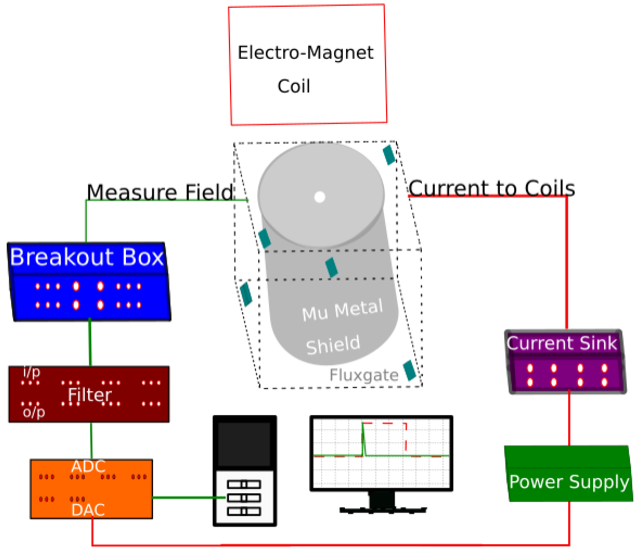
\includegraphics[width=0.4 \textwidth]{Images/exp}
%     \caption[width=0.4 \textwidth]{Schematic diagram of prototype active compensation system at University of Winnipeg . }
%     \label{fig:active shielding}
% \end{figure}
% \begin{figure}
%     \centering
%     \includegraphics[width=0.5 \textwidth]{Images/ss}
%     \caption[width=0.4 \textwidth]{PI loop in flow chart. First measurement from the fluxgates will act as set-point. Then the repeated measurements from the fluxgates are taken. For each measurement difference with the setpoint are noted. On the basis of the difference, the required amount of current for the coils surrounding the outermost layer of the shileding are determined and sent. Those coil currents generate required amount of magnteic flux to compensate for the differences.}
%     \label{fig:active shielding}
% \end{figure}
 The field fluctuations around the prototype has been found tom $\sim \pm$100 nT. It is also discussed that magnetic fields are normally distributed with standard deviation is 1.5 nT. With this section, Chapter~\ref{ch:amcP} is finished.